\section[网中的零空间]{网中的零空间\\Nullspaces for Networks}	
\par \noindent
\emph{Leveling Network (One-Dimensional, Heights Only)}. Incidence matrices take differences of heights. The nullspace contains vectors of constant height
\begin{equation}
	e =
	\begin{pmatrix}
		1,1,...,1
	\end{pmatrix}
\end{equation}
\emph{Two-Dimensional Control Network A translation} of the network in the $x$ direction adds a common constant to all $x$ coordinates. In two dimensions, there can also be a translation in the y direction, and a rigid rotation. If the vector of unknowns is arranged as follows
\begin{equation}
	X =
	\begin{pmatrix}
		X_1,Y_1,X_2,Y_2,...,X_n,Y_n
	\end{pmatrix}
\end{equation}
then the nullspace of $A$ contains $x$ translations and also $y$ translations:
\begin{equation}
	t_x =
	\begin{pmatrix}
		1,0,1,0,...,1,0
	\end{pmatrix}
	\  \text{and}\   t_y =
	\begin{pmatrix}
		0,1,0,1,...,0,1
	\end{pmatrix}.
\end{equation}
Furthermore the network can be \emph{rotated} by an angle $\varphi$. We shall show in detail how to linearize a differential rotation:
\begin{align}
	\begin{split}
		X_{i}^{'} = cos{\varphi}X_i - sin{\varphi}Y_i \\
		Y_{i}^{'} = sin{\varphi}X_i + cos{\varphi}Y_i
	\end{split}
\end{align}
Here $(X_{i},Y_{i})$ is a set of given coordinates which the rotation transforms to $(X_{i}^{'},{Y_{i}^{'}})$.We linearize by $sin{d\varphi} \approx d\varphi$ and $cos{d\varphi} \approx 1$ and keep only the first order terms:
\begin{align*}
	X_{i}^{'} + \varepsilon_i = 1 X_i - d\varphi Y_i\qquad  \varepsilon_i = -Y_i d\varphi   \\
	Y_{i}^{'}  + \eta_i = d\varphi X_i + 1 Y_i\qquad
	\eta_i = X_i d\varphi.
\end{align*}
This small rotation gives rise to yet another vector in the nullspace of $A$:
\begin{equation}
	r_{\varphi} =
	\begin{pmatrix}
		-Y_1,X_1,-Y_2,X_2,...,Y_n,X_n
	\end{pmatrix}.
\end{equation}
Finally \emph{a change in scale $dk$} is described by the vector
\begin{equation}
	s_k =
	\begin{pmatrix}
		X_1,Y_1,X_2,Y_2,...,X_n,Y_n
	\end{pmatrix}.
\end{equation}
Our network is determined up to two translations, one rotation, and one change of scale.The nullspace $\textbf{N}(A)$ is spanned by the four rows of
\begin{equation}
	G^T =
	\begin{bmatrix}
		\color{red} 1&0&1&0&...&1&0\\
		0&1&0&1&...&0&1\\
		-Y_1&X_1&-Y_2&X_2&...&Y_n&X_n\\
		X_1&Y_1&X_2&Y_2&...&X_n&Y_n
	\end{bmatrix}.
\end{equation}
The differential parameters are $df = (dt_x,dt_y,d\varphi,dk)$ and the transformation is
\begin{equation}
	dx =
	\begin{pmatrix}
		\xi_1,\eta_1,...,\xi_n,\eta_n
	\end{pmatrix}
	= G df.
\end{equation}
\textbf{Example 7.1} (Distance measurement) We observe 3 distances in order to locate point P:
\begin{equation}
	f_1 = 100.01\qquad \text{and}\qquad f_2 = 100.02\qquad \text{and}\qquad f_3 = 100.03
\end{equation}
with weights $C = \text{diag}(1,1,1) = I$.Figure 7.1 indicates all preliminary values for the coordinates. As preliminary coordinates for P we use $(\mathbf{X_{P}^{0}},\mathbf{Y_{P}^{0}}) = (170.71, 170.71)$.These values are calculated using simple geometrical relations.
\begin{figure}
	\centering
	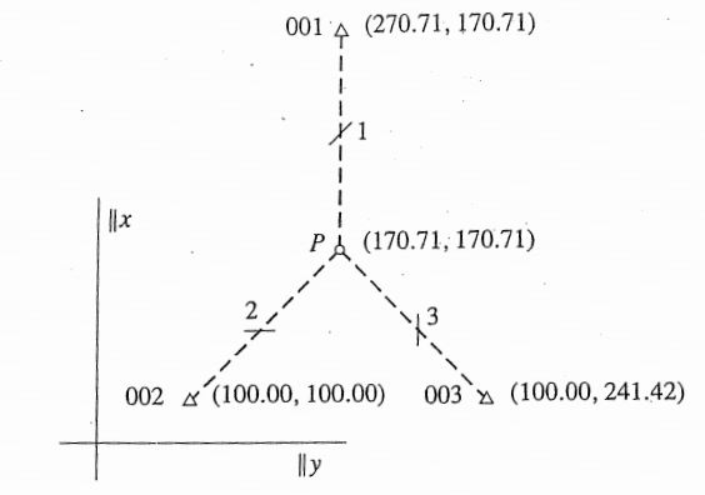
\includegraphics[width=0.4\linewidth]{TeX_files/Part02/chapter07/image/7-1}
	\caption{Figure 7.1 Determining the coordinates of a point by resection}
	\label{fig:7-1}
\end{figure}

\par
The first observation equation is
\begin{equation*}
	\begin{bmatrix}
		- cos{\alpha_{P,001}^{0}} & - sin{\alpha_{P,001}^{0}}
	\end{bmatrix}
	\begin{bmatrix}
		x_P \\ y_P
	\end{bmatrix}
	= f_1 - \sqrt{(X_{001}^{0} - X_{p}^{0})^2 + (Y_{001}^{0} - Y_{p}^{0})^2} - e_1
\end{equation*}
or
\begin{equation*}
	\begin{bmatrix}
		-1 & 0
	\end{bmatrix}
	\begin{bmatrix}
		x_P \\ y_P
	\end{bmatrix}
	= f_1 - 100.000 - e_1,
\end{equation*}
Similarly the second observation equation is
\begin{equation*}
	\begin{bmatrix}
		0.707 1 & 0.7071
	\end{bmatrix}
	\begin{bmatrix}
		x_P \\ y_P
	\end{bmatrix}
	= f_2 - 99.999 - e_2,
\end{equation*}
and finally the third observation equation
\begin{equation*}
	\begin{bmatrix}
		0.707 1 & -0.7071
	\end{bmatrix}
	\begin{bmatrix}
		x_P \\ y_P
	\end{bmatrix}
	= f_3 - 99.999 - e_3,
\end{equation*}
Now all three equations together
\begin{equation*}
	\begin{bmatrix}
		-1 & 0\\
		0.707 1 & 0.7071\\
		0.707 1 & -0.7071
	\end{bmatrix}
	\begin{bmatrix}
		\hat{x}_P \\ \hat{y}_P
	\end{bmatrix}
	= \begin{bmatrix}
		100.01- 100.000\\
		100.02- 99.999\\
		100.03- 99.999
	\end{bmatrix}
	-
	\begin{bmatrix}
		e_1\\
		e_2\\
		e_3
	\end{bmatrix}
\end{equation*}
The normal equations $A^\mathsf{T}A\hat{x} = A^\mathsf{T}b$ are
\begin{equation*}
	\begin{bmatrix}
		2  & 0 \\
		0 & 1
	\end{bmatrix}
	\begin{bmatrix}
		\hat{x}_P \\ \hat{y}_P
	\end{bmatrix}
	=
	\begin{bmatrix}
		0.0267\\
		-0.0071
	\end{bmatrix}.
\end{equation*}
As the coefficient matrix became diagonal(why is $A^\mathsf{T}A$ diagonal in this case?) the solution is easily found as $(\hat{x}_P,\hat{y}_P) = (0.013 4,-0.007 1)$. The final coordinates are $(\hat{X}_P,\hat{Y}_P) = (X_{P}^{0} + \hat{x}_P,Y_{P}^{0} + \hat{y}_P =  (170.723 m, 170.703 m))$.
\par
In this simple example the residuals are most easily calculated as
\begin{equation*}
	\hat{e} = b - A\hat{x}
	= b - P
	=
	\begin{bmatrix}
		0.01 \\ 0.02 \\ 0.03
	\end{bmatrix}
	-
	\begin{bmatrix}
		-0.0127 \\ 0.0040 \\ 0.0140
	\end{bmatrix}
	=
	\begin{bmatrix}
		0.0234 \\ 0.0165 \\ 0.0165
	\end{bmatrix}.
\end{equation*}
Finally ${\hat{\sigma}}_0 = \sqrt{\hat{e}^\mathsf{T}\hat{e}/(3 - 2)} = 0.033m$. The covariance matrix is
\begin{equation*}
	\Sigma_{\hat{x}}
	= {\hat{\sigma}}_{0}^{2}(A^\mathsf{T}A)^{-1}
	=
	\begin{bmatrix}
		0.000514 & 0\\
		0 & 0.001029
	\end{bmatrix}
\end{equation*}
and the standard deviations on the coordinates are $\sigma_{\hat{X}_P} = \sqrt{0.000514} = 0.023$m and $\sigma_{\hat{X}_P} = \sqrt{0.001 029} = 0.033$m.
\par\noindent
\emph{Three-Dimensional Control Network} Three-dimensional networks can be subject to three infinitesimal translations $dt_x,dt_y,dt_z$,three infinitesimal rotations $d\varphi_x,d\varphi_y,d\varphi_z$,and one infinitesimal change of scale $dk$. The nullvectors are the seven rows of
\begin{equation}
	\mathbf{G}^\mathsf{T}
	=
	\begin{bmatrix}
		1 & 0 & 0 \\
		0 & 1 & 0 \\
		0 & 0 & 1 \\
		0 & -Z_1 & Y_1 \\
		Z_1 & 0 & -X_1 \\
		-Y_1 & X_1 & 0 \\
		X_1 & Y_1 & Z_1
	\end{bmatrix}
	\cdots
	\begin{bmatrix}
		1 & 0 & 0 \\
		0 & 1 & 0 \\
		0 & 0 & 1 \\
		0 & -Z_n & Y_n \\
		Z_n & 0 & -X_n\\
		-Y_n & X_n & 0 \\
		X_n & Y_n & Z_n
	\end{bmatrix}
\end{equation}
with
\begin{equation}
	d\mathsf{f}
	=
	\begin{pmatrix}
		dt_x,dt_y,dt_z,d\varphi_x,d\varphi_y,d\varphi_z \\
	\end{pmatrix}
\end{equation}
The columns of G (rows of $G^\mathsf{T}$) span $N(A)$ and we have
\begin{equation}
	AG = 0.
\end{equation}
We close this section by suggesting a geometrical interpretation. The first three rows of $G^\mathsf{T}x = 0$ means that the origin is fixed. For numerical reasons we translate the origin
to the barycenter and provide coordinates $(X^\ast,Y^\ast,Z^\ast)$relative to the barycenter:
\begin{equation*}
	\sum_{i=1}^{n}X^\ast = 0,\qquad\sum_{i=1}^{n}Y^\ast = 0,\qquad\sum_{i=1}^{n}Z^\ast = 0.
\end{equation*}
The next three equations in $G^\mathsf{T}x = g$ lead to rotations:
\begin{equation*}
	\sum_{i=1}^{n}(-Y_{i}^{\ast}\varepsilon_i + X_{i}^{\ast}\eta_i) = g_4,\qquad
	\sum_{i=1}^{n}( Z_{i}^{\ast}\varepsilon_i - X_{i}^{\ast}\zeta_i) = g_5\qquad
	\sum_{i=1}^{n}(-Z_{i}^{\ast}\eta_i        + Y_{i}^{\ast}\zeta_i) = g_6.
\end{equation*}
The final condition $\sum_{n=1}^n(X_{i}^{\ast}\varepsilon_i + Y_{i}^{\ast}\eta_i + Z_{i}^{\ast}\zeta_i)$ secures that scale is kept fixed.
\par\noindent
\textbf{Table 7.1} Possible $G$-columns spanning the nullspace of $A$, see Teunissen (1985a). The number of unknowns at each node is denoted $u$ , and $d$ is the dimension of $N(A)$.
\begin{center}
	\begin{tabular}{cccccccccc}
		\hline
		\multirow{2}{*}{$u$}& \multirow{2}{*}{$d$} & \multirow{2}{*}{Observation type(s)} & \multicolumn{7}{c}{Components of $G$-column(s)} \\
		\cline{4-10}
		\multicolumn{3}{c}{}    &  \multicolumn{3}{c}{translation(s)} &  \multicolumn{3}{c}{rotation (s)} & scale(s)\\
		\hline
		1 & 1 & height differences & &1\\
		\hline
		\multirow{2}{*}{} & \multirow{2}{*}{2}  & \multirow{2}{*}{distances and azimuths} &1&0\\
		\multicolumn{3}{c}{} &0&1\\
		\\
		\multirow{2}{*}{2} & \multirow{2}{*}{3} & \multirow{2}{*}{distances} &1 &0&&& \quad$Y_i$\\
		\multicolumn{3}{c}{} &0&1&&& $-X_i$\\
		\\
		\multirow{2}{*}{} & \multirow{2}{*}{4} & \multirow{2}{*}{angles and/or distance ratios} &1 &0&&& \quad$Y_i$ &&$X_i$\\
		\multicolumn{3}{c}{} &0&1&&& $-X_i$&&$Y_i$\\
		\hline
		\multirow{3}{*}{} & \multirow{3}{*}{3} & distances, azimuths, &1&0&0\\
		\multicolumn{2}{c}{} &astronomical latitudes and&0&1&0\\
		\multicolumn{2}{c}{} &longitudes&0&0&1\\
		\\
		\multirow{3}{*}{3} & \multirow{3}{*}{6} & \multirow{3}{*}{distances} &1&0&0 &\quad0&$-Z_i$&\quad$Y_i$\\
		\multicolumn{3}{c}{} &0&1&0&\quad$Z_i$&\quad0&$-X_i$\\
		\multicolumn{3}{c}{} &0&0&1&$-Y_i$&\quad$X_i$&\quad0\\
		\\
		\multirow{3}{*}{} & \multirow{3}{*}{7} & \multirow{3}{*}{angles and/or distance ratios} &1&0&0 &\quad0&$-Z_i$&\quad$Y_i$&$X_i$\\
		\multicolumn{3}{c}{} &0&1&0&\quad$Z_i$&\quad0&$-X_i$&$Y_i$\\
		\multicolumn{3}{c}{} &0&0&1&$-Y_i$&\quad$X_i$&\quad0&$Z_i$\\
		\hline
	\end{tabular}
\end{center}